\chapter{Background}
\label{chap:ch2}

\indent\par Informatii si citare carte \cite{Sommerville2010}.

\section{Methods used}
\label{sec:ch2sec1}

\par Methods/algorithms used in programming and training chess engines.

\section{State of the art chess engines}
\label{sec:ch2sec2}

\par Stockfish, AlphaZero etc. - overview and AI techniques used in them 

% Informatii si citare articol publicat la conferinta (in proceedings) \cite{Narayan2012}.

% Informatii si citare articol publicat în revista \cite{Robbes2015}.

% Informatii si citare articol publicat tip masterthesis  \cite{mastersthesis1993}.

% Informatii si citare articol publicat tip phdthesis \cite{phdthesis1993}.

% Informatii si citare articol ca resursa Internet  \cite{kinaSUR}.

% Inserarea si Referirea unei figuri \ref{FigCBSD}.

% \begin{figure}[htbp]
% 	\centering
% 		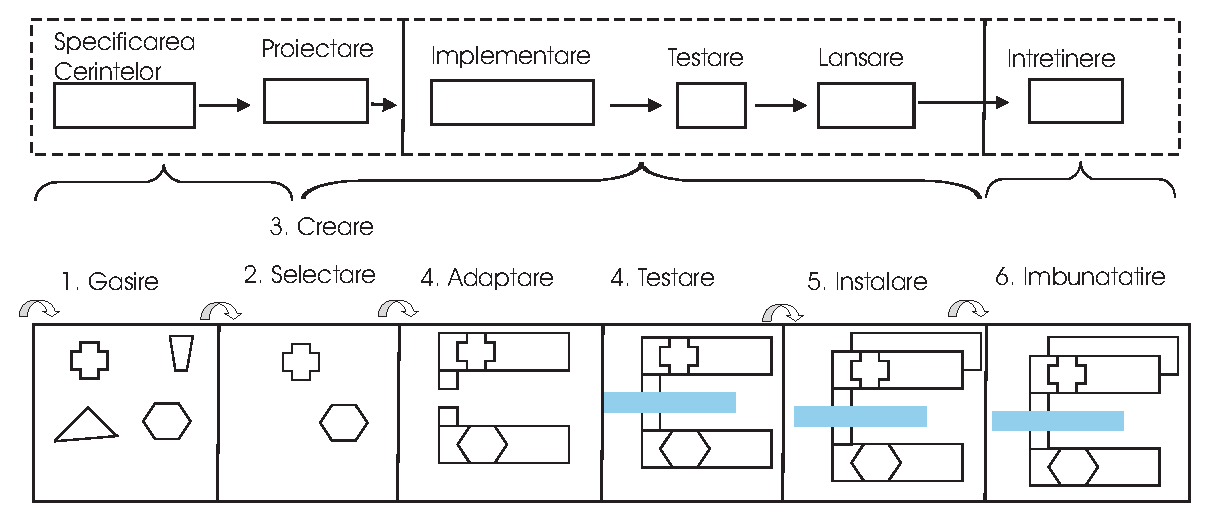
\includegraphics[scale=0.65]{./figures/fig_3_1.eps}
% 	\caption{Ciclul de dezvoltare al sistemelor bazate pe componente adaptat modelului cascadã}
% 	\label{FigCBSD}
% \end{figure}

% Inserarea si Referirea la Tabelul \ref{TabelSolutii}.

% \begin{table}[htbp]
% \begin{center}
% \begin{tabular}
% {|p{120pt}|p{120pt}|p{120pt}|}
% \hline
%  Nume algoritm  &  Toate solutiile &  Solutia optimã\\
% \hline 
% \hline Nume 1 & $20$ & $5$  \\
% \hline Nume 2 & $20$ & $2$  \\
% \hline
% \end{tabular}
% \end{center}
% \caption{Solutii obtinute }
% \label{TabelSolutii}
% \end{table}

% Adaugarea si Referirea la o Ecuatie \ref{LabelMyEquation}.

%  \begin{equation}
%      ws_N4 = w_{14}*N1 + W_{24}+N2 + w_{34}*N3
% \label{LabelMyEquation}
%  \end{equation}
 
